\documentclass[8pt]{article}
\usepackage{amsfonts}
\usepackage{amsmath}
\usepackage{mathtools}
\usepackage{graphicx}
\usepackage{float}
\usepackage{pythonhighlight}
\usepackage[all]{foreign}
\usepackage{cleveref}
\usepackage{fmtcount}
\usepackage{verbatim}
\usepackage{multicol}
\usepackage{xparse}

\NewDocumentCommand\weight{}{\textsf{weight}\xspace}

\title{Probabilistic Logic Programming Exam}
\author{
        Francesco Fabiano, Luca Geatti\\
        \footnotesize Department of Mathematics, Computer Science and Physics \\
        \footnotesize University of Udine\\
        \footnotesize via delle Scienze, 206, 33100 Udine, \underline{Italy}
}
\date{\footnotesize\today}


\begin{document}
\maketitle
\paragraph{Abstract}
This is a report for the exam of the PhD course on Probabilistic Logic
Programming, held at University of Udine in the academic year 2018-2019.



\section{Introduction}

  \paragraph{The problem}
    Modern \textit{biometrics}-based tool exploit the fact that these biometric characteristics, used for the verification of an individual’s identity, are unique from person to person.
    That is way the majority of the studies in this filed aim to generate biometric tools that are able to distinguish even twins.
    
    The purpose of these researches is to identify the uniqueness of each \textit{fingerprint}, facial feature or others characteristics of a person.
    For all these reasons, to the best of our knowledge, no study exists that tries to exploit heredity in such features.
    \textit{Heredity} may be defined as the transmission of characteristics from the parents to the offspring.
    Such traits as body size, hair color, skin color, eye color, etc. are known to be inherited.
    The cell is the unit of structures and the unit of heredity.
    Chromosomes in all of the body cells of a single individual are alike.
    Thus, the individual functions as a single unit—alike in every cell yet different from all other people.
    
    In this study we try to extrapolate from a fingerprint, the most used biometric characteristics, a data structure informative enough to be used for heredity-finding purposes.
    This newly created data structure will be defined starting from the fingerprint \textit{minutiae}, informative points of the fingerprint itself often used for the \textquoteleft classical' biometrics-based recognition (The circles in Figure~\ref{fig:ske_min}).
%\paragraph{Fare un' introduzione su PLP.}
  \paragraph{Exploiting P.L.P.}
    The main idea of the study, as said before, is to capture a new fingerprint description starting from the widely used minutiae.
    This new structure can be pictured as a directed \textit{graph} with some constrains on the edges: each node can have at most one \textit{incoming edge} and at most two \textit{outgoing}.
    The main idea behind this graph (shown in Figure~\ref{fig:ske_min_graph}) is that it should \textquoteleft emulate' the \textit{skeleton} (the black lines of Figure~\ref{fig:ske_min}) of the fingerprint.
    As reconstructing this graph could be somewhat trivial when in posses of the fingerprint's original image, it is not when the only available information are the fingerprint's minutiae.
    Unfortunately this is the case in most of the official databases where, due to space optimization, the fingerprints are only stored as a set of minutiae along with few other information.
    
   	\begin{figure}
    	\centering
    	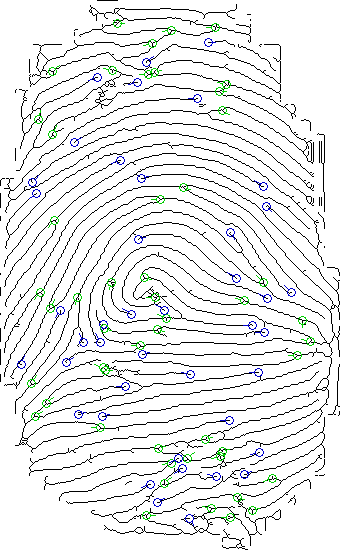
\includegraphics[width=0.35\linewidth]{img/ske_min}
    	\caption{The skeleton and the minutiae of a fingerprint.}
    	\label{fig:ske_min}
    \end{figure}
    
    \begin{figure}
    	\centering
    	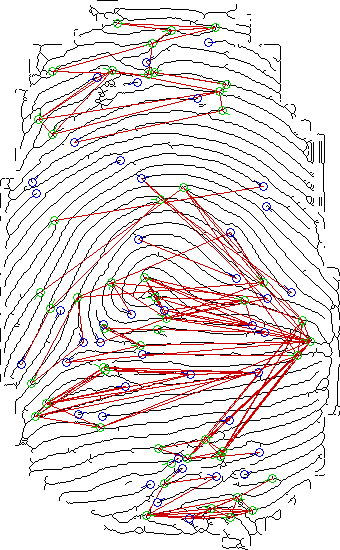
\includegraphics[width=0.35\linewidth]{img/ske_min_graph}
    	\caption{The ideal graph of the fingerprint in Figure~\ref{fig:ske_min}.}
    	\label{fig:ske_min_graph}
    \end{figure}%
    
    This is way we decided to exploit \textit{Probabilistic Logic Programming}.
   	In fact, having the fingerprints regular patterns (Figure~\ref{fig:patterns}), we could exploit this information to reconstruct the graph using probability.
   	In particular our aim is to associate each edge with a percentage of existence based on various factors such as: length, angle, position, crossing with other edges, incoming and outgoing nodes.
   	Once that all the edges have been labeled the result will be a probabilistic graph that could be used as base for heredity-base recognition.
   	Through the use of P.L.P. it has been possible to characterize probabilistic constraints that allowed the graph reconstruction.
   	As further step we though to exploit the \textquoteleft learning' capabilities of this paradigm allowing the program to infer the best weight for each constraints relative to each pattern.

    \begin{figure}
		\centering
		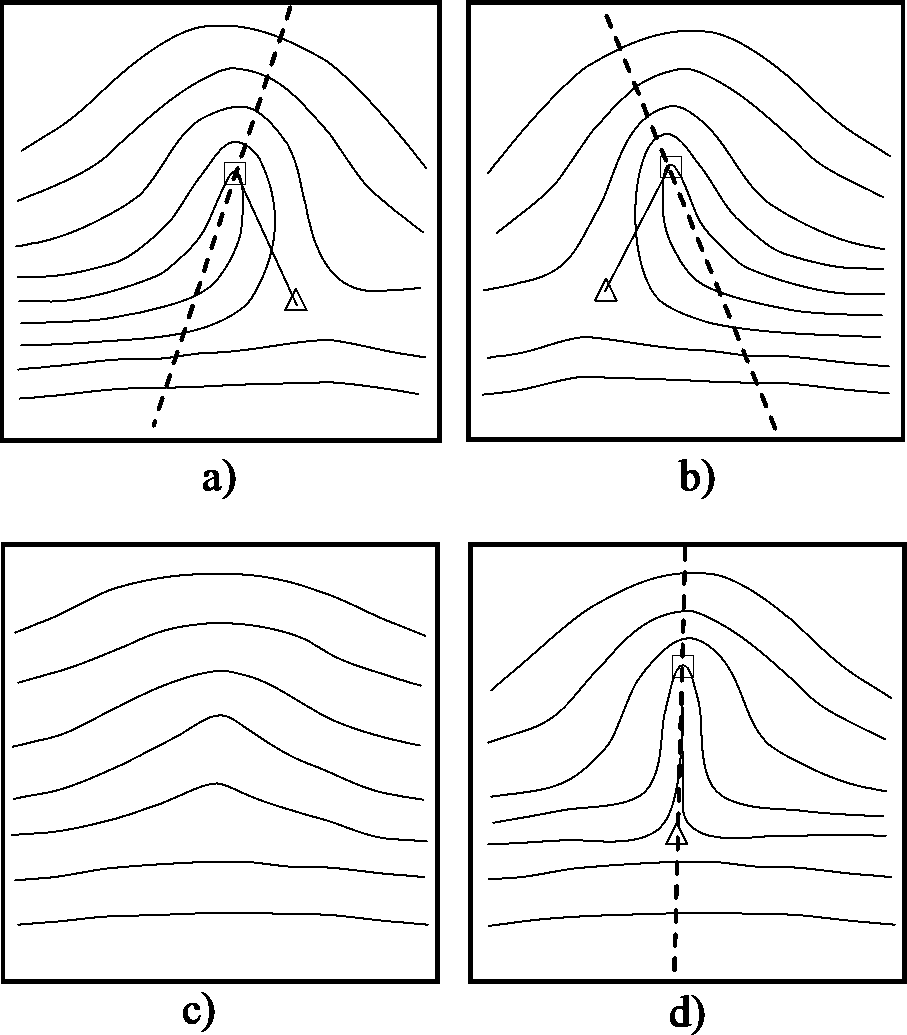
\includegraphics[width=0.6\linewidth]{img/patterns}
		\caption{Fingerprint patterns as they appear at a coarse level: a) \textit{left loop}, b) \textit{right loop}, c) \textit{\textit{arch}}, and d) tented arch; squares denote loop-type singular points, and triangles
			delta-type singular points..}
		\label{fig:patterns}
	\end{figure}%





%%%%%%%%%%%%%%%%%%%%%%%%%%%%%%%%%%%%%%%%%%%%%%%%%%%%%%%
%%% Encoding
%%%%%%%%%%%%%%%%%%%%%%%%%%%%%%%%%%%%%%%%%%%%%%%%%%%%%%%
\section{Encoding}
\label{sec:encoding}
We start by describing the basic predicates we introduced to model
the problem. In order to model a minutia, we introduced the predicate
  \begin{center}
    \textsf{minutia(X,Y,D,T)}
  \end{center}
where $\textsf{X},\textsf{Y} \in \mathbb{N}$ are the coordinates of the minutiae 
inside the image along the X-axis and Y-axis, respectively;
$\textsf{D} \in [0,2\pi]$ is the direction, expressed in radians; 
and $T \in \{e,b\}$ is the type of the fingerprint ($e$ stands for
\emph{ending}, $b$ for \emph{bifurcation}).
The second predicate is
  \begin{center}
    \textsf{type\_fingerprint(T)}
  \end{center}
where $\textsf{T}\in\{
  \textsf{tented\_archs},
  \textsf{plain\_archs},
  \textsf{left\_loop},
  \textsf{right\_loop},
  \textsf{whorl}
\}$; 
basically, it express which type the overall fingerprint belongs to.
Finally, \textsf{max\_X(N)} and \textsf{max\_Y(N)} express the number
of pixels of the image along the X-axis and the Y-axis, respectively.
The \emph{knowledge base} of our program will be the set of all the 
\textsf{minutia/4} predicates corresponding to the input file,
the \textsf{type\_fingerprint/1} predicate and the \textsf{max\_X/1}
and \textsf{max\_Y/1} predicates.

Since what we want to entail are the edges between the minutiae along
with their probability of existence, we introduced the predicate
  \begin{center}
    \textsf{edge($X_1,Y_1,X_2,Y_2$)}
  \end{center}
where $(X_1,Y_1)$ are the coordinates of one end and $(X_2,Y_2)$
the coordinate of the other end.
Since in our setting we want undirected edges (their direction doesn't
matter), some simmmetry breaking constraints can be added to the 
encoding, aiming at removing specular but equivalent solutions; in
particular, we constrained that there must exists only left-to-right
edges.

\subsection{Structure constraints}
We introduce two structure constraints to forbid wrong edges
in the final solution.
\paragraph{Constraint 1}:
each B-minutia has exactly $3$ incident edges. This has been achieved
using the \texttt{aggregate\_all} predicate.
\paragraph{Constraint 2}:
similarly, each E-minutia has exactly $2$ incident edges.


\section{Probability constraints}
\subsection{Tented Archs}
\paragraph{Contraint TA1}:
Given two E-minutiae belonging to a tented arch fingerprint, we note that 
the probability of existence of an edge between these two minutiae 
is high if they have opposite directions and low if the have 
the same direction.
Let $M_1=(X_1,Y_1,D_1,e)$ and $M_2=(X_2,Y_2,D_2,e)$ be two E-minutiae.
Let 
  \begin{align*}
    \weight_d(M_1,M_2) \coloneqq 
    \frac{
      \left( \pi - \Big\lvert \lvert D_1-D_2 \rvert - 
      \pi \rvert\Big\rvert \right)}{\pi}
  \end{align*} 
The more $\lvert D_1-D_2 \rvert$ is close to $\pi$ (resp. $0$), the more 
$weight_d(M_1,M_2)$ is close to $1$ (resp. $0$).
With Constraint TA1, we give the value $weight_d(M_1,M_2)$ to the probability 
of existence of an edge between $M_1$ and $M_2$.



\paragraph{Contraint TA2}:
Given two B-minutiae belonging to a tented arch fingerprint, the more
these two minutiae are distant (either in the x-axis or in the y-axis)
the less an edge between them is likely to exists.

Let $M_1=(X_1,Y_1,D_1,b)$ and $M_2=(X_2,Y_2,D_2,b)$ be two B-minutiae.
Let $max_x$ and $max_y$ be the maximum value for the x-coordinate and
y-coordinate, respectively. We define:
  \begin{align*}
    \weight_x(M_1,M_2) \coloneqq
    \frac{\lvert X_1 - X_2 \rvert}{max_x}
  \end{align*}
  \begin{align*}
    \weight_y(M_1,M_2) \coloneqq
    \frac{\lvert Y_1 - Y_2 \rvert}{max_y}
  \end{align*}
We give the value $\weight_x$ and $\weight_y$ to the probability 
of existence of an edge between $M_1$ and $M_2$.




\subsection{Plain Archs}
Tutti i vincoli uguali a Tented Archs, piu TA5 con ended e tranne "uno meno".


\subsection{Left/Right Loop}
Non dividiamo in 4 quadranti, ma piuttosto diamo un peso a tutte le
regole, cioè sia a quelle standard dei plain archs (due quadranti superiori)
sia a quelle specifiche per i left/right loops (due quadranti inferiori).

I pesi per le probabilità sono opposti per i due tipi di regole, a seconda
che si avvicinino o meno alla parte bassa o alta dell'immagine. L'idea è
questa:
  \begin{itemize}
    \item
      piu mi avvicino alla parte bassa dell'immagine e piu do peso alle
      regole per i left/right loops. Faccio questo \emph{moltiplicando}
      la probabilita dell'arco per il valore:
        \begin{align*}
          1 - Y_1 \cdot Y_2
        \end{align*}
    \item
      similmente, piu mi avvicino alla parte alta dell'immagine e piu 
      do peso alle regole per i plain archs.
  \end{itemize}









\end{document}
